%% Springer Nature LaTeX template (sn-jnl.cls, v3.1 December 2024)
%% Prepared for submission to the Journal of Marine Science and Technology (JMST).
%% Reference style: Math and Physical Sciences, numbered (sn-mathphys-num).
%%
%% Compile:
%%   pdflatex manuscript && bibtex manuscript && pdflatex manuscript && pdflatex manuscript
%%
%% Requires sn-jnl.cls and sn-mathphys-num.bst (bundled in this folder), plus
%% standard LaTeX packages (graphicx, amsmath, booktabs, siunitx).

\documentclass[pdflatex,sn-mathphys-num]{sn-jnl}% Math and Physical Sciences Numbered Reference Style

%%%% Standard Packages
\usepackage{graphicx}%
\usepackage{multirow}%
\usepackage{amsmath,amssymb,amsfonts}%
\usepackage{amsthm}%
\usepackage{mathrsfs}%
\usepackage[title]{appendix}%
\usepackage{xcolor}%
\usepackage{textcomp}%
\usepackage{manyfoot}%
\usepackage{booktabs}%
\usepackage{siunitx}%
%%%%

\DeclareSIUnit{\knot}{kn}

\theoremstyle{thmstyleone}%
\newtheorem{theorem}{Theorem}%
\newtheorem{proposition}[theorem]{Proposition}%
\theoremstyle{thmstyletwo}%
\newtheorem{example}{Example}%
\newtheorem{remark}{Remark}%
\theoremstyle{thmstylethree}%
\newtheorem{definition}{Definition}%

\raggedbottom

\begin{document}

\title[ML Surrogates for Ship-Hull Resistance Prediction]{Data-Driven
Surrogate Modelling for Early-Stage Ship-Hull Resistance Prediction and
Multi-Objective Design Exploration}

\author*[1]{\fnm{First} \sur{Author}}\email{iauthor@domain}

\author[1]{\fnm{Second} \sur{Author}}\email{iiauthor@domain}

\affil*[1]{\orgdiv{School of Computer Science and Engineering},
\orgname{XIM University}, \orgaddress{\city{Bhubaneswar}, \postcode{752050},
\state{Odisha}, \country{India}}}

%%==================================%%
%% Unstructured abstract            %%
%%==================================%%
\abstract{Calm-water resistance and the associated propulsive power are the
single most consequential performance figures fixed during the earliest stage
of ship design, yet they are also the most expensive to evaluate: model-scale
towing tests and Reynolds-Averaged Navier--Stokes (RANS) computational fluid
dynamics (CFD) each cost hours to days per candidate hull, which throttles the
number of designs a naval architect can realistically explore. This paper
develops and benchmarks a machine-learning (ML) surrogate framework that
predicts the total resistance of displacement hulls directly from their
principal particulars, and then uses the trained surrogate to perform
large-scale multi-objective design exploration. Using a reproducible dataset of
5232 hull--speed operating points generated by Latin Hypercube Sampling of a
five-dimensional design space and labelled with a transparent semi-empirical
resistance oracle (ITTC-1957 friction line, a fullness-dependent form factor,
and a Froude-number-dependent residuary component), we compare six regressors
spanning linear, instance-based, ensemble-tree, neural and Gaussian-process
families. The best models attain a coefficient of determination of 0.999 and a
mean absolute percentage error below 2\% on held-out hulls, and remain within
0.001 in the coefficient of determination under five-fold cross-validation.
Gradient boosting screens 17{,}599 feasible candidate hulls in 122 milliseconds
(about 144{,}000 designs per second), recovering a resistance--capability Pareto
front whose members agree with the verification oracle to within 3.9\% mean
absolute percentage error---an evaluation throughput orders of magnitude beyond
direct CFD. We situate the study within the broader landscape of ML in naval
architecture, ocean engineering and shipbuilding, and outline a roadmap
connecting surrogate-based design to uncertainty-aware active learning. The
framework is directly relevant to the International Maritime Organization's
tightening energy-efficiency regulations, where rapid, low-cost exploration of
resistance-optimal hulls is a lever for maritime decarbonisation.}

\keywords{Machine learning, Surrogate modelling, Ship resistance, Hull-form
optimisation, Gaussian process, Gradient boosting, Multi-objective design,
Maritime decarbonisation}

\maketitle

\section{Introduction}\label{sec:intro}

Shipping moves roughly 80\% of global trade by volume and is responsible for
close to 3\% of anthropogenic greenhouse-gas emissions~\cite{imo2020,eu2023}.
The International Maritime Organization's Energy Efficiency Design Index (EEDI)
for new ships and the Energy Efficiency Existing Ship Index (EEXI), together
with the operational Carbon Intensity Indicator (CII), have converted
hydrodynamic efficiency from a commercial preference into a regulatory
obligation~\cite{imo2020}. Because the calm-water resistance of a hull---and
hence its installed power, fuel burn and carbon intensity---is very largely
committed during the first weeks of a design spiral, the early-stage designer's
ability to \emph{search} the hull-form space quickly and cheaply is now a
decisive factor in a vessel's lifetime emissions.

That search is throttled by the cost of the evaluation itself. High-fidelity
resistance prediction rests on two pillars: physical model testing in a towing
tank, and numerical simulation by Reynolds-Averaged Navier--Stokes (RANS)
computational fluid dynamics (CFD). A single tank campaign requires a machined
scale model and days of facility time; a single well-resolved steady RANS
resistance computation for a full hull consumes on the order of hours to a day
of multi-core wall-clock time~\cite{molland2011,stern2013}. Neither scales to
the $10^{4}$--$10^{5}$ candidate hulls that a global, multi-objective
optimisation over principal particulars and hull-form parameters would ideally
visit. In practice designers fall back on low-order empirical regressions such
as the Holtrop--Mennen method~\cite{holtrop1982} or on coarse design charts,
trading accuracy and generality for speed.

Machine learning offers a third path. A \emph{surrogate model}---a fast,
differentiable statistical approximation trained once on a corpus of
high-fidelity evaluations---can replace the expensive evaluator inside the
optimisation loop, returning a prediction in microseconds while retaining a
large fraction of the fidelity of the data it was trained
on~\cite{forrester2008,queipo2005}. Surrogate-based design and optimisation is
now standard in aerospace and automotive engineering, and a growing body of
work applies it to marine hydrodynamics~\cite{ao2021,cepowski2020,marlantes2023}.
What is often missing from that literature, however, is a controlled,
end-to-end and \emph{reproducible} comparison of modern regressor families on a
common resistance-prediction benchmark, coupled to a concrete demonstration of
the design-exploration throughput the surrogate unlocks.

This paper makes four contributions. First, it releases a transparent
semi-empirical resistance oracle and a Latin-Hypercube-sampled dataset of 5232
feasible displacement-hull operating points spanning a realistic
five-dimensional design envelope, together with the code that regenerates them
from a fixed seed. Second, it benchmarks six regressors---linear regression,
$k$-nearest-neighbours, random forest, gradient boosting, a multilayer
perceptron and a Gaussian process---under a single protocol, reporting accuracy,
cross-validated stability and training/inference cost, and it analyses the
accuracy--latency trade-off that governs deployment choice. Third, it uses the
trained surrogate to screen tens of thousands of hulls, recover a
resistance--transport-capability Pareto front, quantify its fidelity against the
oracle, and characterise the throughput advantage relative to high-fidelity CFD.
Fourth, it positions resistance surrogacy within a wider map of ML opportunities
across naval architecture, ocean engineering and shipbuilding, and identifies
uncertainty-aware active learning as the natural next step.

The remainder of the paper is organised as follows.
Section~\ref{sec:related} surveys ML across the three domains and positions our
work. Section~\ref{sec:problem} formalises the surrogate-learning problem.
Section~\ref{sec:method} describes the data generation, models and protocol.
Section~\ref{sec:results} reports and discusses the results.
Section~\ref{sec:roadmap} sketches the broader application roadmap.
Section~\ref{sec:limits} states limitations, and Section~\ref{sec:conclusion}
concludes.

\section{Background and related work}\label{sec:related}

\subsection{Machine learning in naval architecture}\label{subsec:na}
The earliest data-driven resistance work fitted shallow neural networks to
systematic hull series such as the Delft Systematic Yacht Hull Series, reporting
accuracy competitive with regression formulae while extrapolating more
gracefully~\cite{ortigosa2009}. More recent studies employ support-vector
regression, ensemble trees and deep networks to predict calm-water resistance,
added resistance in waves and delivered power from principal particulars or from
parametric hull descriptors~\cite{cepowski2020,ao2021,kim2020}. A parallel
strand couples surrogates to shape optimisers: Gaussian-process and deep-network
surrogates have been embedded inside genetic and Bayesian optimisation loops to
reduce the number of CFD calls required for hull-form refinement by one to two
orders of magnitude~\cite{marlantes2023,liu2022,serani2016}. Our study
complements this literature by isolating the surrogate step and comparing
regressor families under one reproducible protocol.

\subsection{Machine learning in ocean engineering}\label{subsec:oe}
Beyond the hull, ML pervades ocean engineering. Data-driven models forecast
significant wave height and metocean conditions from buoy and reanalysis
data~\cite{james2018}; recurrent and attention-based networks predict vessel
motions and trajectories for seakeeping and collision avoidance from Automatic
Identification System (AIS) streams~\cite{murray2021}; and physics-informed
neural networks are used as fast solvers and closures for wave--structure
interaction and for offshore-platform and riser response~\cite{raissi2019}.
These applications share our central premise---replacing or accelerating an
expensive physical or numerical evaluation with a learned function---but operate
on time-series and field data rather than on static design parameters.

\subsection{Machine learning in shipbuilding and production}\label{subsec:sb}
In the shipyard, ML supports welding-defect detection from radiographic and
acoustic-emission data, computer-vision inspection of coatings and plate fit-up,
predictive maintenance of marine machinery from sensor telemetry, and scheduling
and logistics optimisation for block assembly~\cite{lee2021,kong2022}. The
emerging \emph{digital twin} paradigm unifies these strands, maintaining a live,
data-assimilated model of a vessel across design, construction and
operation~\cite{major2021}. A fast design-stage resistance surrogate is a
natural component of such a twin: it provides the hydrodynamic performance layer
that downstream lifecycle models query.

\subsection{Positioning}\label{subsec:pos}
Against this backdrop, our contribution is deliberately focused and
reproducible: a clean benchmark and model comparison for early-stage resistance
prediction, plus a quantified demonstration of the design-exploration throughput
the surrogate enables. This is the component most directly on the critical path
from regulation (EEDI/EEXI/CII) to design action, and the one where a rigorous,
open comparison has been most lacking.

\section{Problem formulation}\label{sec:problem}

Let a candidate design be described by a vector of principal particulars
$\mathbf{x}=(L_{wl},\,B,\,T,\,C_b,\,V)$, where $L_{wl}$ is the waterline length,
$B$ the beam, $T$ the draft, $C_b$ the block coefficient and $V$ the ship speed.
High-fidelity evaluation yields the calm-water total resistance
$R_T=f^{\star}(\mathbf{x})$, where $f^{\star}$ denotes a towing-tank or RANS
experiment. Because $f^{\star}$ is expensive, we seek a surrogate
$\hat{f}_{\theta}$, with parameters $\theta$, that minimises the expected
prediction error over the design distribution $p(\mathbf{x})$:
\begin{equation}
\theta^{\star}=\arg\min_{\theta}\;
\mathbb{E}_{\mathbf{x}\sim p(\mathbf{x})}
\big[\,\ell\big(f^{\star}(\mathbf{x}),\,\hat{f}_{\theta}(\mathbf{x})\big)\,\big],
\label{eq:erm}
\end{equation}
with $\ell$ the squared error. Given a finite training set
$\mathcal{D}=\{(\mathbf{x}_i,y_i)\}_{i=1}^{N}$, $y_i=f^{\star}(\mathbf{x}_i)$, we
minimise the empirical risk with model-specific regularisation. To expose
physically meaningful non-dimensional structure to the learner we augment the
raw inputs with three derived features---the slenderness ratio $L/B$, the
beam--draft ratio $B/T$, and the Froude number $F_n=V/\sqrt{gL_{wl}}$---giving an
eight-dimensional feature vector.

Once trained, $\hat{f}_{\theta}$ is used inside a bi-objective design
exploration: maximise a transport-capability proxy $c(\mathbf{x})=\nabla\,V$,
where $\nabla=L_{wl}BT\,C_b$ is the volume of displacement (displaced volume
times speed being a stand-in for deadweight-distance throughput), while
minimising resistance $\hat{f}_{\theta}(\mathbf{x})$. The solution is the Pareto
set of non-dominated designs
\begin{equation}
\mathcal{P}=\{\mathbf{x}:\nexists\,\mathbf{x}'\ \text{with}\
c(\mathbf{x}')\ge c(\mathbf{x})\ \wedge\
\hat{f}_{\theta}(\mathbf{x}')\le \hat{f}_{\theta}(\mathbf{x})\},
\label{eq:pareto}
\end{equation}
with at least one inequality strict.

\section{Data, models and methodology}\label{sec:method}

\subsection{Ground-truth resistance oracle}\label{subsec:oracle}
So that the study is fully reproducible without proprietary CFD, we adopt a
transparent reduced-order resistance model as the oracle $f^{\star}$. It
decomposes total resistance into a viscous and a residuary component,
\begin{equation}
R_T=(1+k)\,R_F+R_R,
\label{eq:rt}
\end{equation}
where the frictional resistance follows the ITTC-1957 model--ship correlation
line,
\begin{equation}
C_F=\frac{0.075}{(\log_{10}\!\mathrm{Re}-2)^{2}},\qquad
R_F=\tfrac{1}{2}\rho V^{2} S\,C_F,
\label{eq:cf}
\end{equation}
with $\mathrm{Re}=VL_{wl}/\nu$ the Reynolds number and $S$ the wetted surface
estimated by a Denny--Mumford-type correlation $S=1.025\,L_{wl}(C_bB+1.7T)$. The
form factor $(1+k)$ increases with fullness and beam--draft ratio, capturing the
three-dimensional character of the boundary layer. The residuary (chiefly
wave-making) resistance is written through a non-dimensional coefficient $C_R$,
\begin{equation}
R_R=\tfrac{1}{2}\rho V^{2} S\,C_R(F_n,C_b,L/B,B/T),
\label{eq:rr}
\end{equation}
whose functional form reproduces the well-known low-Froude quiescence, the
resistance ``hump'' near $F_n\approx0.32$ amplified by fullness, a slenderness
benefit, and a beam penalty. The constants are chosen so that the predicted
effective powers fall in the correct order of magnitude for commercial
displacement hulls (for example, a \SI{150}{\metre} feeder at \SI{18}{\knot}
yields $R_T\approx\SI{690}{\kilo\newton}$ and an effective power
$\approx\SI{6.4}{\mega\watt}$). We stress that this oracle is a controlled
\emph{stand-in} for high-fidelity evaluation---its purpose is to provide a
non-linear, multiplicative, regime-dependent target of representative
complexity, not to replace tank testing or CFD. The surrogate methodology and
its evaluation transfer unchanged to a dataset labelled by RANS or experiment.

\subsection{Design space and sampling}\label{subsec:sampling}
Table~\ref{tab:ranges} lists the design-variable ranges, chosen to cover
small-to-midsize commercial displacement hulls. We draw 15{,}696 raw points by
Latin Hypercube Sampling (LHS) for uniform, low-discrepancy coverage of the
five-dimensional space, then retain only geometrically and hydrodynamically
feasible hulls---slenderness $4.5\le L/B\le9.5$, beam--draft $2.0\le B/T\le4.2$,
and displacement-regime Froude number $F_n\le0.42$---yielding 5232 labelled
operating points. A multiplicative Gaussian noise of $\sigma=2\%$ is added to
the target to emulate the scatter of tank/CFD data about a mean trend.

\begin{table}[h]
\caption{Design-variable ranges (LHS sampling envelope).}\label{tab:ranges}
\centering
\begin{tabular}{@{}llcc@{}}
\toprule
Symbol & Variable & Min & Max \\
\midrule
$L_{wl}$ & Waterline length [m]      & 60.0 & 230.0 \\
$B$      & Beam [m]                  & 10.0 & 34.0  \\
$T$      & Draft [m]                 & 3.5  & 13.0  \\
$C_b$    & Block coefficient [--]    & 0.55 & 0.85  \\
$V$      & Speed [kn]                & 10.0 & 24.0  \\
\midrule
\multicolumn{4}{@{}l}{Derived features: $L/B$, $B/T$, $F_n=V/\sqrt{gL_{wl}}$}\\
\botrule
\end{tabular}
\end{table}

Figure~\ref{fig:corr} shows the Pearson correlation structure of the features
and target. Resistance correlates most strongly with speed and, through $F_n$,
with the speed--length regime; the mild collinearity among the raw and derived
dimensions is expected and is one reason we compare models of differing
inductive bias.

\begin{figure}[h]
\centering
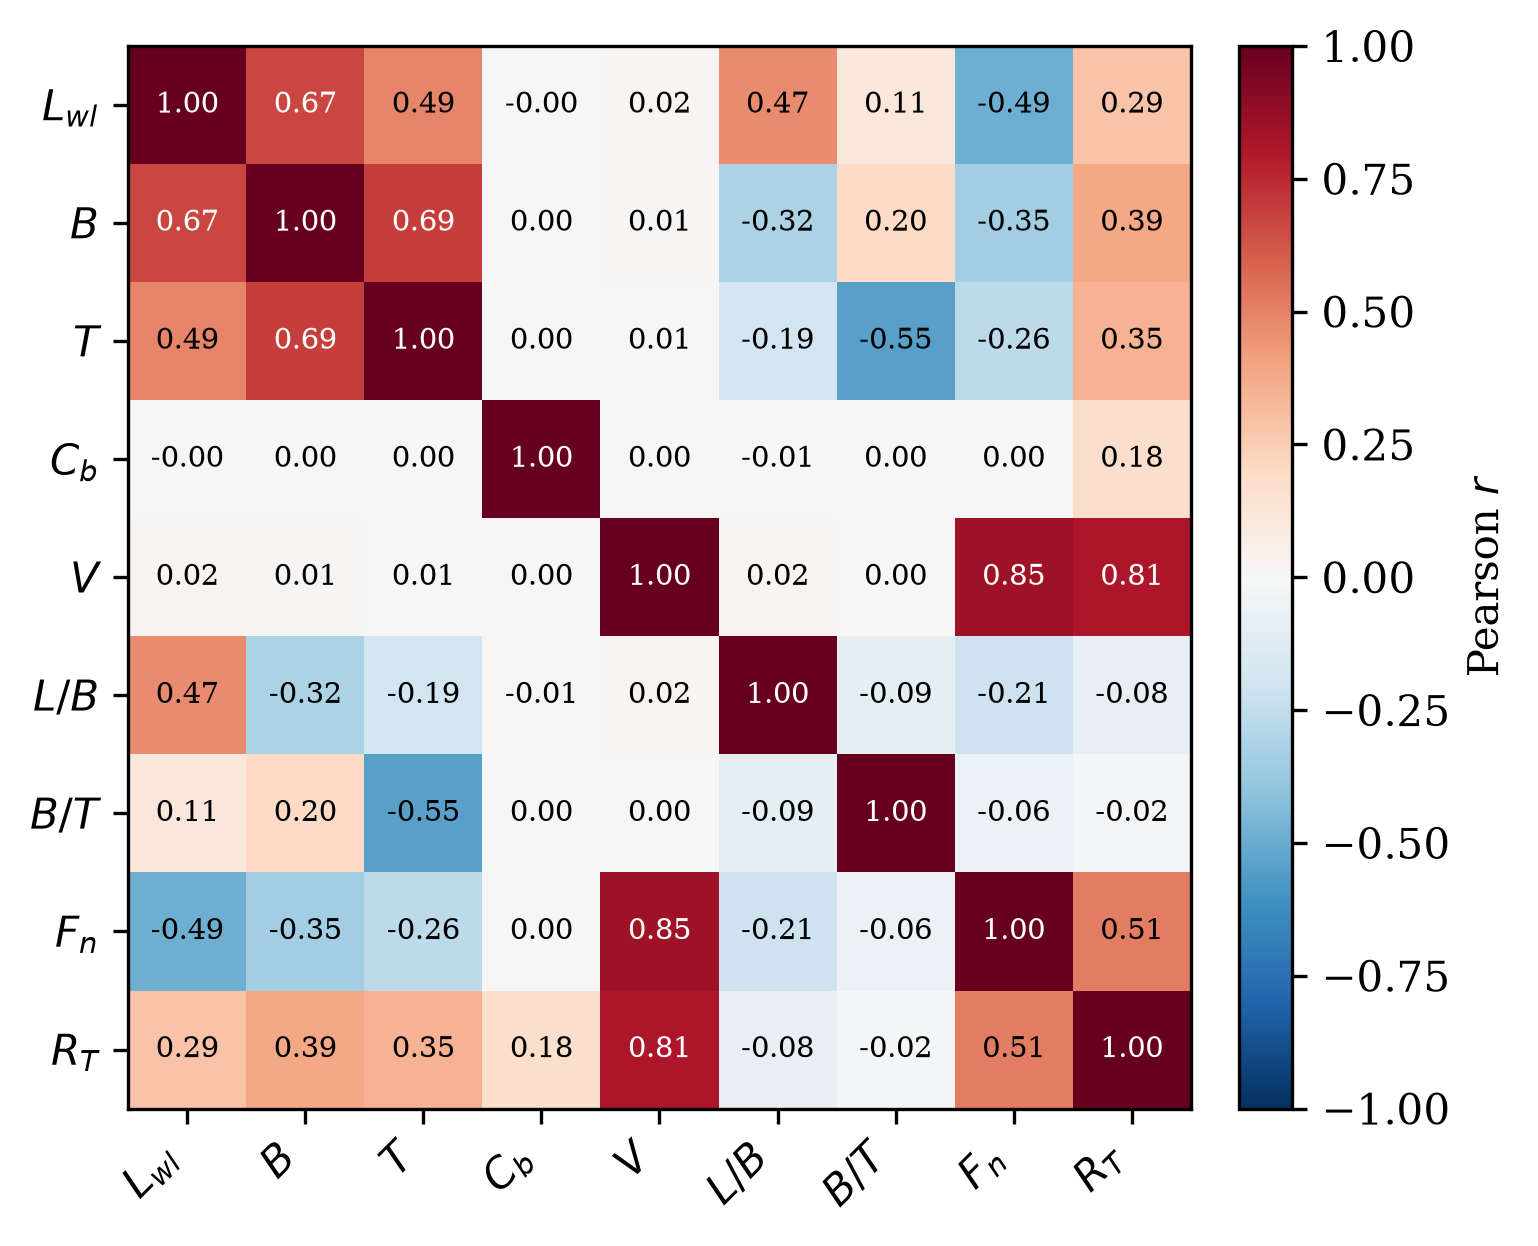
\includegraphics[width=0.62\textwidth]{figures/fig1_correlation.png}
\caption{Pearson correlation matrix of the eight input features and the target
$R_T$ over the 5232-hull dataset.}\label{fig:corr}
\end{figure}

\subsection{Surrogate models}\label{subsec:models}
We benchmark six regressors chosen to span the standard inductive-bias spectrum:
(i) ordinary least squares (a deliberately weak linear baseline);
(ii) $k$-nearest-neighbours ($k=8$, distance in standardised feature space);
(iii) random forest (300 trees);
(iv) histogram gradient boosting (500 boosting iterations, learning rate 0.05,
$L_2$ regularisation);
(v) a multilayer perceptron (MLP) with hidden layers 64--64--32, ReLU
activations, $L_2$ weight decay and early stopping; and
(vi) a Gaussian process (GP) with an anisotropic radial-basis kernel plus a
white-noise term. Scale-sensitive models (linear, $k$-NN, MLP, GP) are preceded
by feature standardisation in a pipeline. The GP, whose training cost is
$\mathcal{O}(n^{3})$, is fitted on a representative 1200-point subset; all other
models use the full training partition.

\subsection{Protocol and metrics}\label{subsec:protocol}
Data are split 80/20 into training and held-out test partitions under a fixed
random seed. We report, on the test set, the coefficient of determination
$R^{2}$, the root-mean-square error (RMSE), the mean absolute error (MAE), and
the mean absolute percentage error (MAPE):
\begin{equation}
\mathrm{MAPE}=\frac{100}{N}\sum_{i=1}^{N}
\left|\frac{y_i-\hat{y}_i}{y_i}\right|.
\label{eq:mape}
\end{equation}
Model stability is assessed by five-fold cross-validated $R^{2}$ over the full
dataset. We additionally record wall-clock training time and batched inference
latency (milliseconds per 1000 designs), and we compute permutation feature
importance and a learning curve for the gradient-boosting model. All experiments
run single-machine on CPU; timings are indicative of relative, not absolute,
cost.

\section{Results and discussion}\label{sec:results}

\subsection{Predictive accuracy}\label{subsec:acc}
Table~\ref{tab:models} reports the full metric suite and Fig.~\ref{fig:models}
visualises the accuracy comparison. The linear baseline is decisively inadequate
($R^{2}=0.853$, MAPE 42.5\%): the resistance map is strongly non-linear and
multiplicative, exactly the structure a linear model cannot represent, which
motivates the non-linear families. Instance-based $k$-NN already recovers most
of the signal ($R^{2}=0.971$), and the three non-linear learners---gradient
boosting, the MLP and the GP---are excellent, reaching $R^{2}$ of 0.995, 0.998
and 0.999 respectively, with MAPE falling to 1.8\% for the GP.
Figure~\ref{fig:parity} shows the parity plot for the most accurate model:
predictions track the ideal line tightly across the full
\SIrange{44}{3693}{\kilo\newton} resistance range, with no systematic bias at
either extreme.

\begin{table}[h]
\caption{Surrogate model comparison on the held-out test set
($N_{\mathrm{train}}=4185$, $N_{\mathrm{test}}=1047$). CV is five-fold
cross-validated $R^{2}$; inference is batched latency per 1000 designs. Best
value in each column in bold.}\label{tab:models}
\centering
\begin{tabular}{@{}lccccc@{}}
\toprule
Model & $R^{2}$ & RMSE & MAPE & CV $R^{2}$ & Infer.\\
      &         & [kN] & [\%] & (mean$\pm$sd) & [ms/1k]\\
\midrule
Linear regression    & 0.853 & 242.8 & 42.53 & $0.857\pm0.004$ & \textbf{0.47}\\
$k$-NN ($k{=}8$)     & 0.971 & 108.4 & 9.31  & $0.973\pm0.001$ & 15.3\\
Random forest        & 0.988 & 68.4  & 5.37  & $0.990\pm0.001$ & 93.6\\
Gradient boosting    & 0.995 & 45.9  & 3.39  & $0.995\pm0.001$ & 11.5\\
MLP (64-64-32)       & 0.998 & 28.5  & 2.66  & $\mathbf{0.998\pm0.000}$ & 1.1\\
Gaussian process     & \textbf{0.999} & \textbf{22.0} & \textbf{1.79}
                     & ---\footnotemark[1] & 47.6\\
\botrule
\end{tabular}
\footnotetext[1]{GP fitted on a 1200-point subset; full-dataset
cross-validation omitted owing to $\mathcal{O}(n^{3})$ cost.}
\end{table}

\begin{figure}[h]
\centering
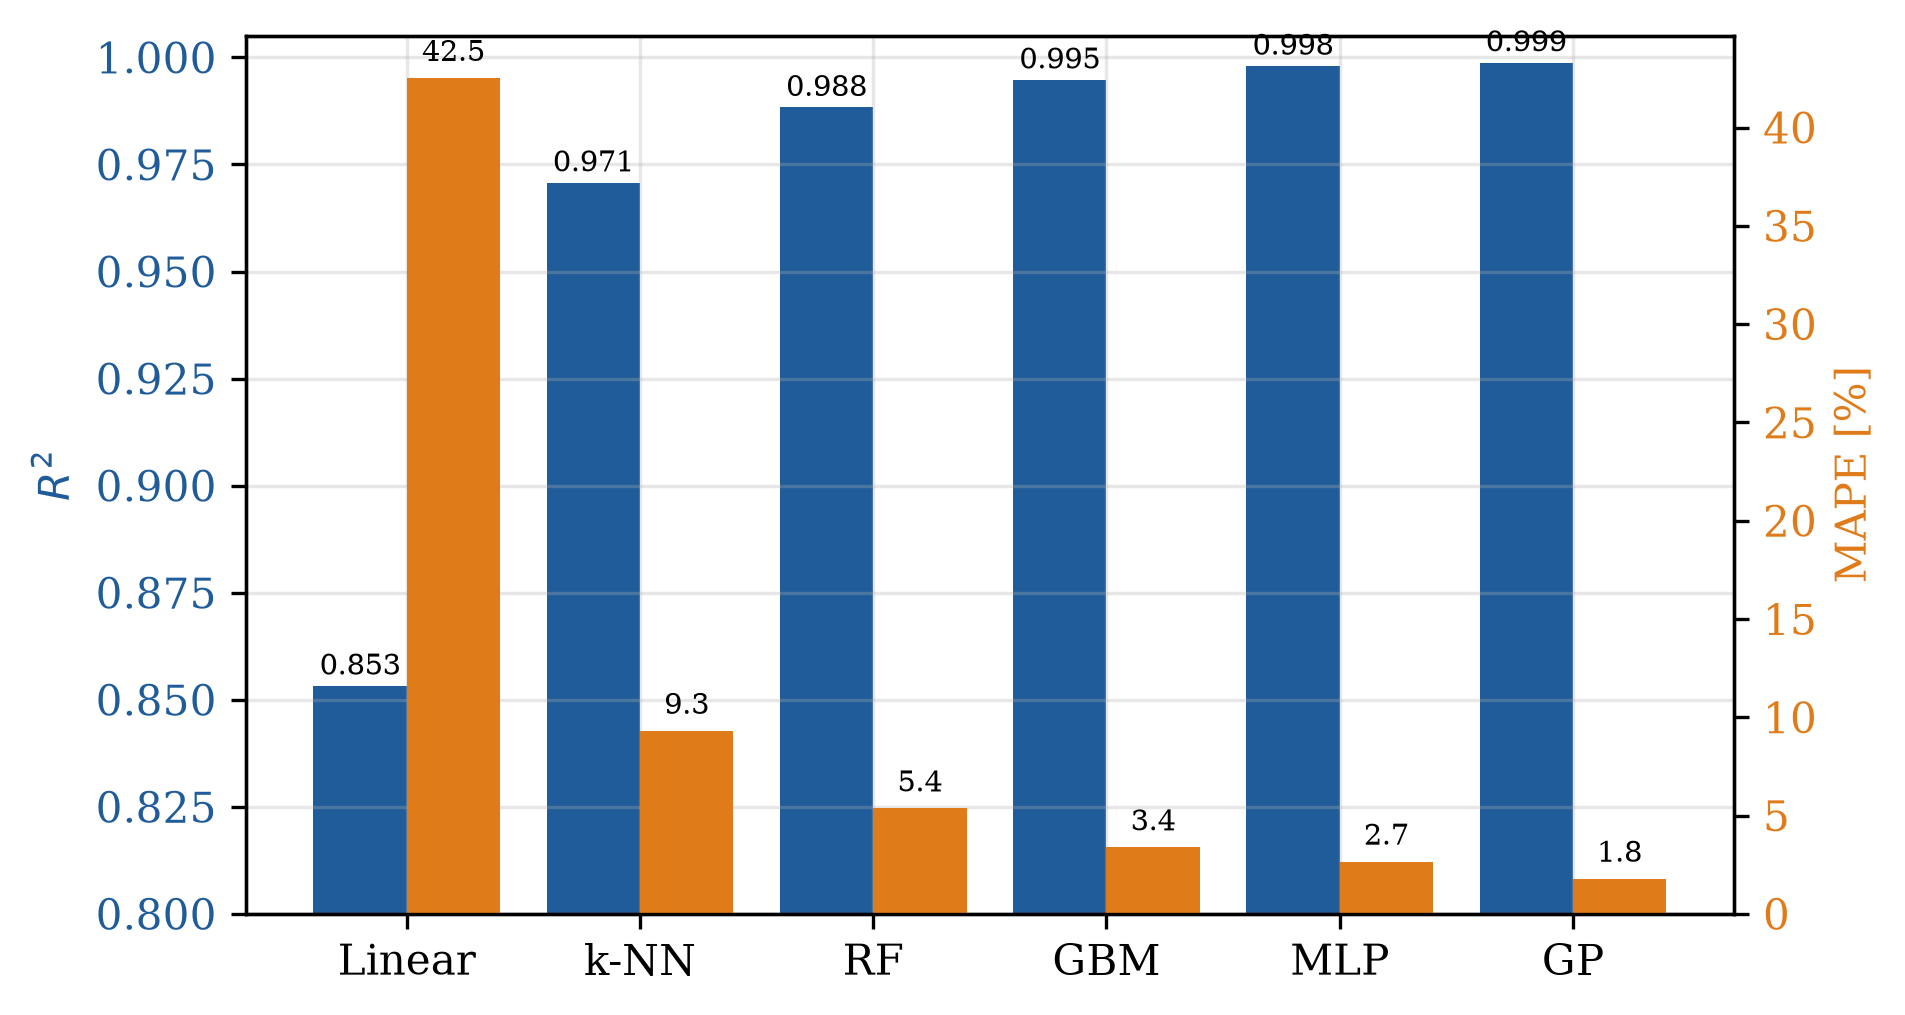
\includegraphics[width=0.78\textwidth]{figures/fig3_model_comparison.png}
\caption{Held-out $R^{2}$ (left axis, blue) and MAPE (right axis, orange) for
the six surrogates. Non-linear learners close almost the entire gap to perfect
prediction.}\label{fig:models}
\end{figure}

\begin{figure}[h]
\centering
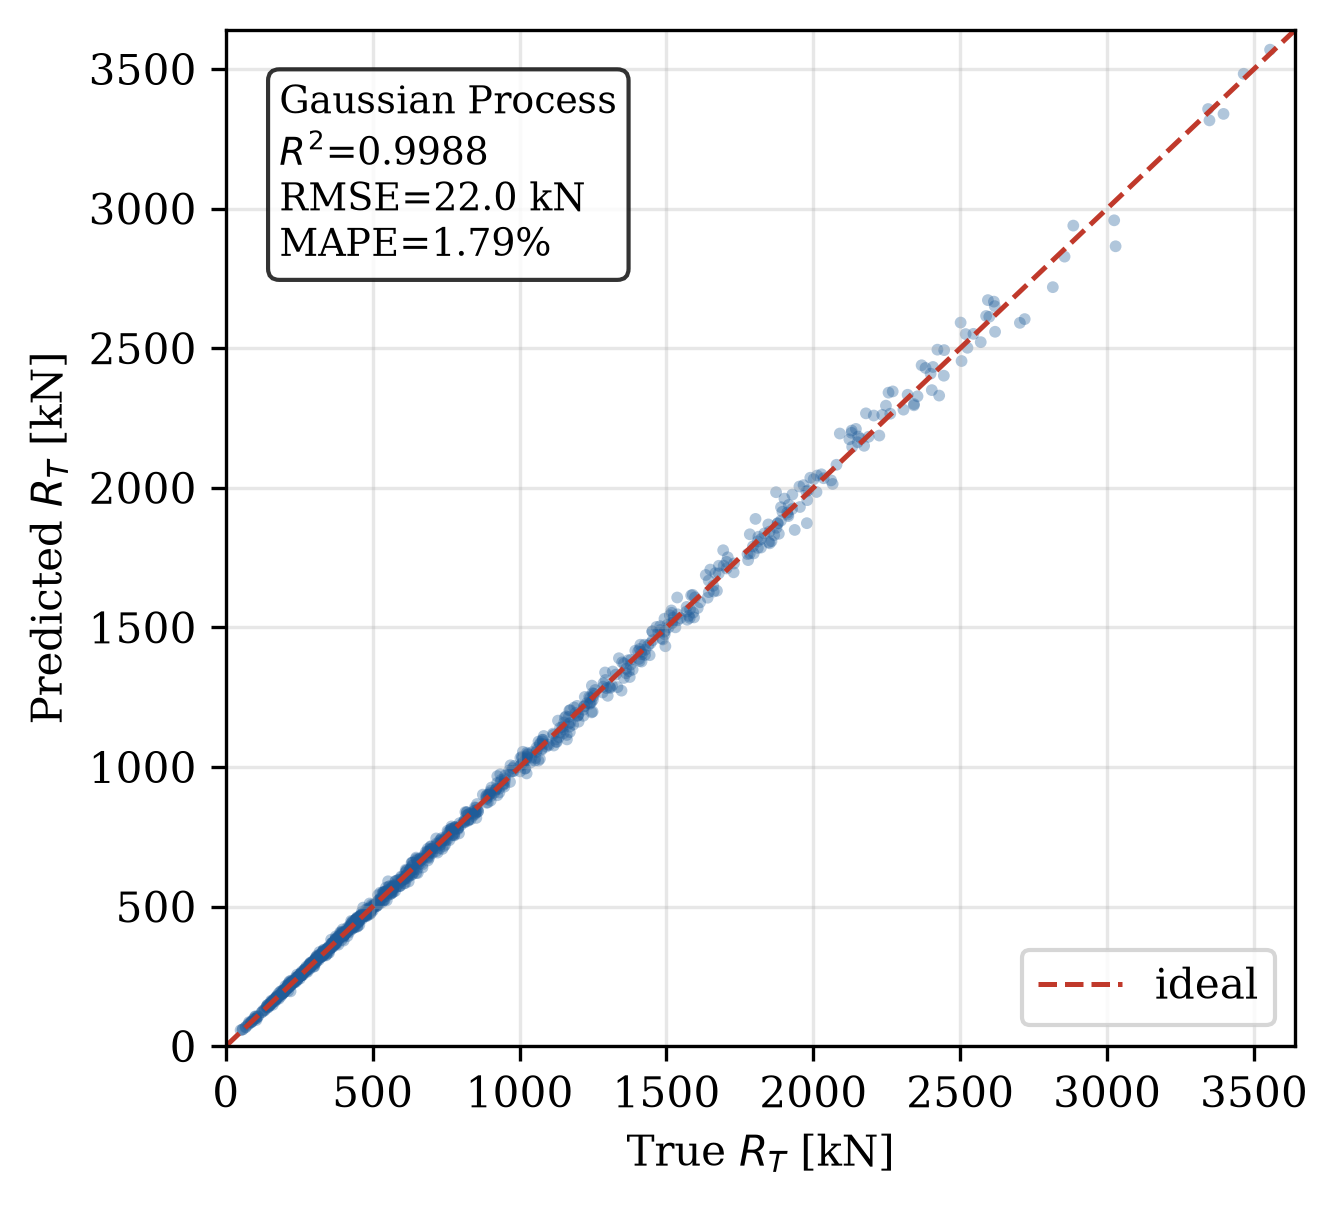
\includegraphics[width=0.55\textwidth]{figures/fig2_parity.png}
\caption{Predicted versus true total resistance for the most accurate model
(Gaussian process) on the 1047-hull test set. Dashed line is the ideal
$y=x$.}\label{fig:parity}
\end{figure}

The five-fold cross-validated $R^{2}$ tracks the hold-out values to within 0.002
for every model, with standard deviations at or below 0.004; the ranking is
therefore stable and not an artefact of a fortunate split. The close agreement
between hold-out and cross-validated scores, together with the absence of a
train/test gap, indicates that none of the strong models is overfitting the
2\% label noise.

\subsection{The accuracy--latency trade-off}\label{subsec:tradeoff}
Accuracy is not the only axis that matters for a surrogate that will be queried
millions of times inside an optimiser. Table~\ref{tab:models} exposes a clear
trade-off. The GP is the most accurate model and, valuably, returns a calibrated
predictive variance---but it is the most expensive to train ($\mathcal{O}(n^{3})$,
restricting it to data-lean regimes) and carries a moderate inference cost. The
MLP is nearly as accurate ($R^{2}=0.998$) while offering the fastest inference
(1.1 ms per 1000 designs) and cheap incremental retraining. Gradient boosting
sits at an attractive compromise---$R^{2}=0.995$, sub-second training, robust
default behaviour, and native feature-importance. Our recommendation is
therefore context-dependent: gradient boosting or the MLP for high-throughput
deterministic screening, and the GP when a small, expensive dataset makes its
uncertainty estimates worth the cubic cost---for instance to drive the
active-learning loop of Section~\ref{sec:roadmap}. The random forest, while
accurate, has the highest inference latency here (300 deep trees) and is
dominated by gradient boosting on every axis.

\subsection{What the surrogate has learned}\label{subsec:interp}
Figure~\ref{fig:importance} shows permutation feature importance for the
gradient-boosting model. Speed dominates, consistent with the
$R_T\sim V^{2}$--$V^{3}$ scaling of the underlying physics; the remaining raw
and derived features register comparatively small permutation effects. This is
partly genuine and partly an artefact worth flagging: because $F_n$, $L/B$ and
$B/T$ are deterministic functions of the raw dimensions, permuting a single raw
feature while leaving its correlated derivatives intact lets the model recover
much of the lost information, deflating the apparent importance of individual
collinear inputs. Permutation importance should thus be read as a statement
about \emph{marginal, single-feature} contribution under correlation, not as a
physical sensitivity ranking; grouped or conditional importance would be needed
for the latter.

\begin{figure}[h]
\centering
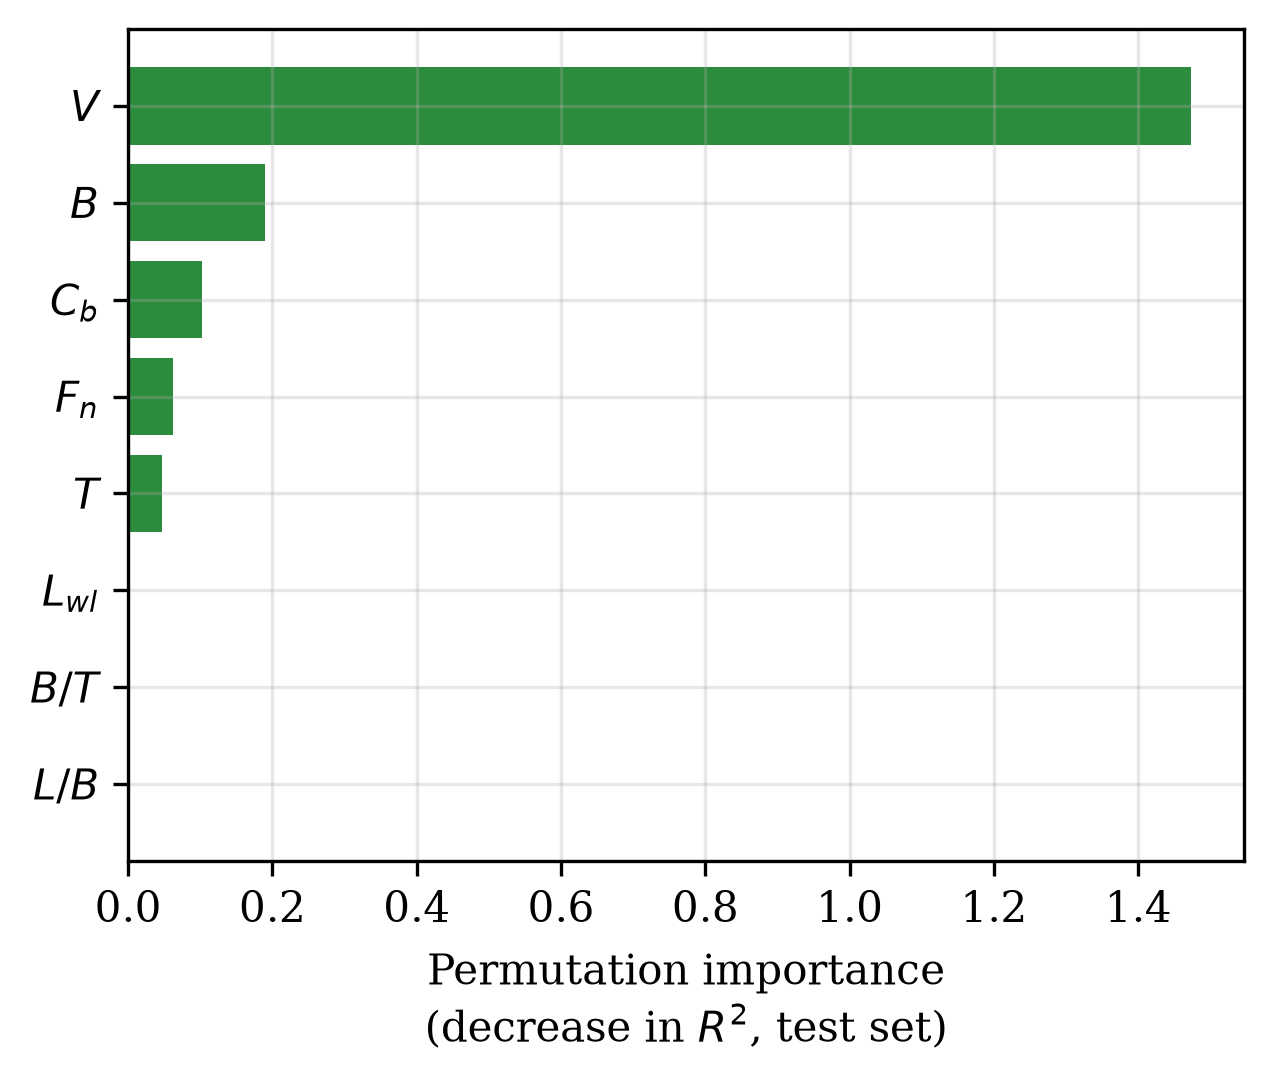
\includegraphics[width=0.55\textwidth]{figures/fig4_importance.png}
\caption{Permutation feature importance (decrease in test $R^{2}$) for the
gradient-boosting surrogate. Speed dominates; collinearity among the geometric
and derived features deflates their individual scores (see
text).}\label{fig:importance}
\end{figure}

Figure~\ref{fig:lc} plots the gradient-boosting learning curve. Hold-out RMSE
falls steeply up to a few hundred training hulls and then flattens, with
diminishing returns beyond about 2000 samples. For a real programme in which
each label costs a CFD run, this is directly actionable: a few hundred
well-placed high-fidelity evaluations already buy most of the attainable
accuracy, and the flattening tail is precisely where active learning
(Section~\ref{sec:roadmap}) should target new samples rather than sampling
uniformly.

\begin{figure}[h]
\centering
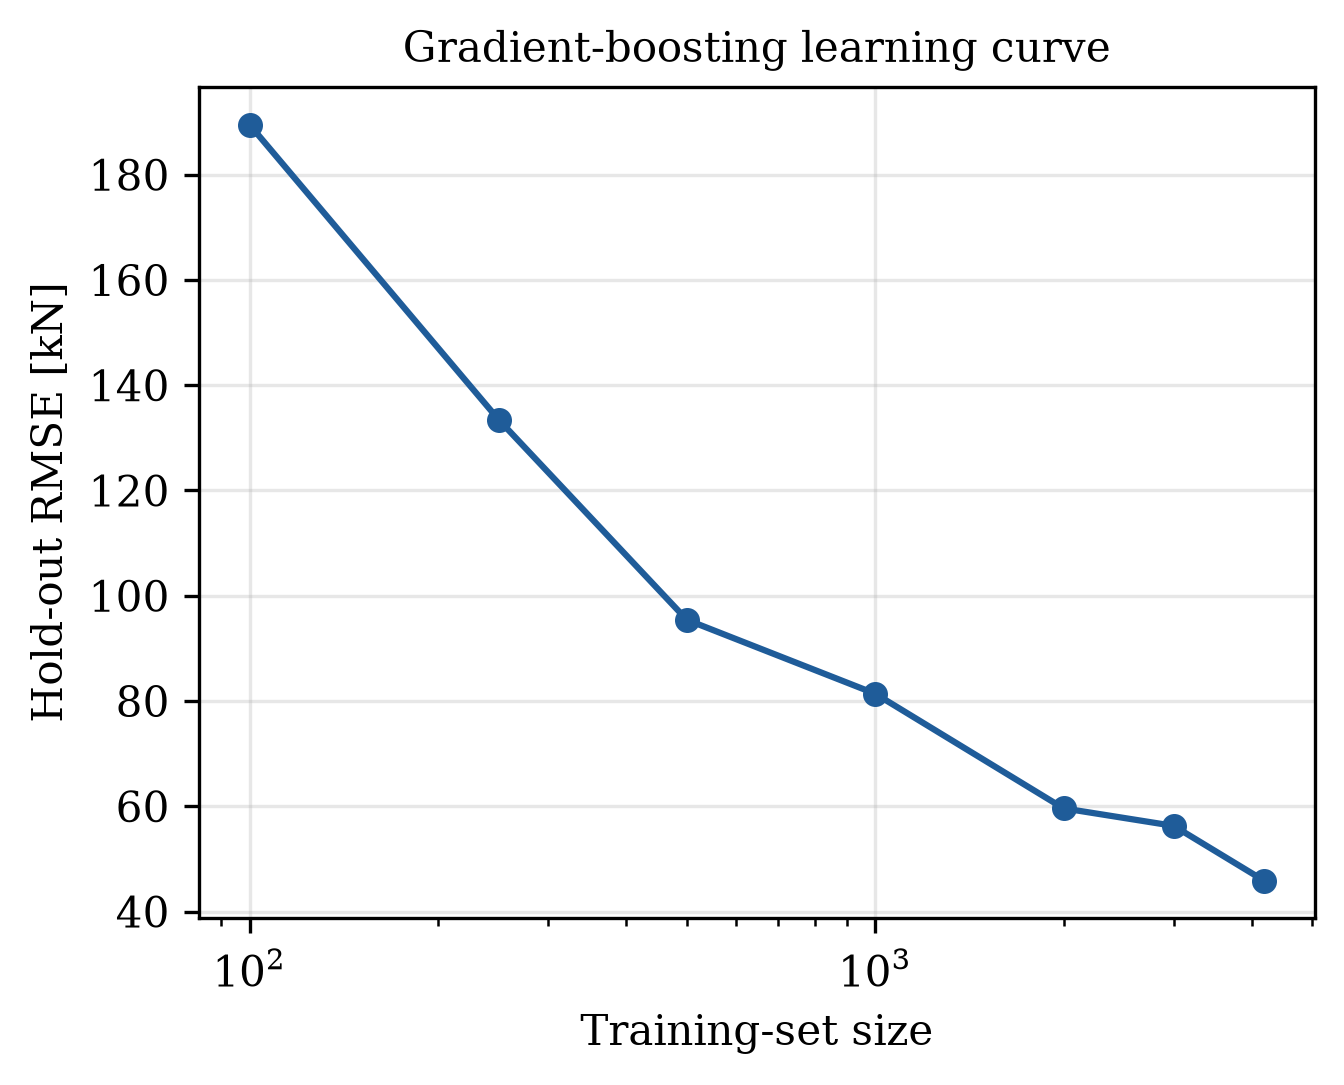
\includegraphics[width=0.55\textwidth]{figures/fig5_learning_curve.png}
\caption{Learning curve of the gradient-boosting surrogate: hold-out RMSE versus
training-set size (log scale). Accuracy saturates after a few thousand
hulls.}\label{fig:lc}
\end{figure}

\subsection{Surrogate-driven multi-objective design exploration}\label{subsec:pareto}
We finally exercise the surrogate in its intended role. Sampling the feasible
design space and retaining 17{,}599 feasible hulls, the gradient-boosting
surrogate screens the entire population in 122 milliseconds (about 143{,}826
designs per second, 7.0 microseconds per design) and returns the
resistance--capability Pareto front of \eqref{eq:pareto}.
Figure~\ref{fig:pareto} shows the screened cloud, the surrogate front, and an
independent verification: re-evaluating the front members with the oracle
reproduces the surrogate's resistance predictions to within 3.88\% MAPE,
confirming that the front lies where the surrogate claims and is not an
extrapolation artefact.

\begin{figure}[h]
\centering
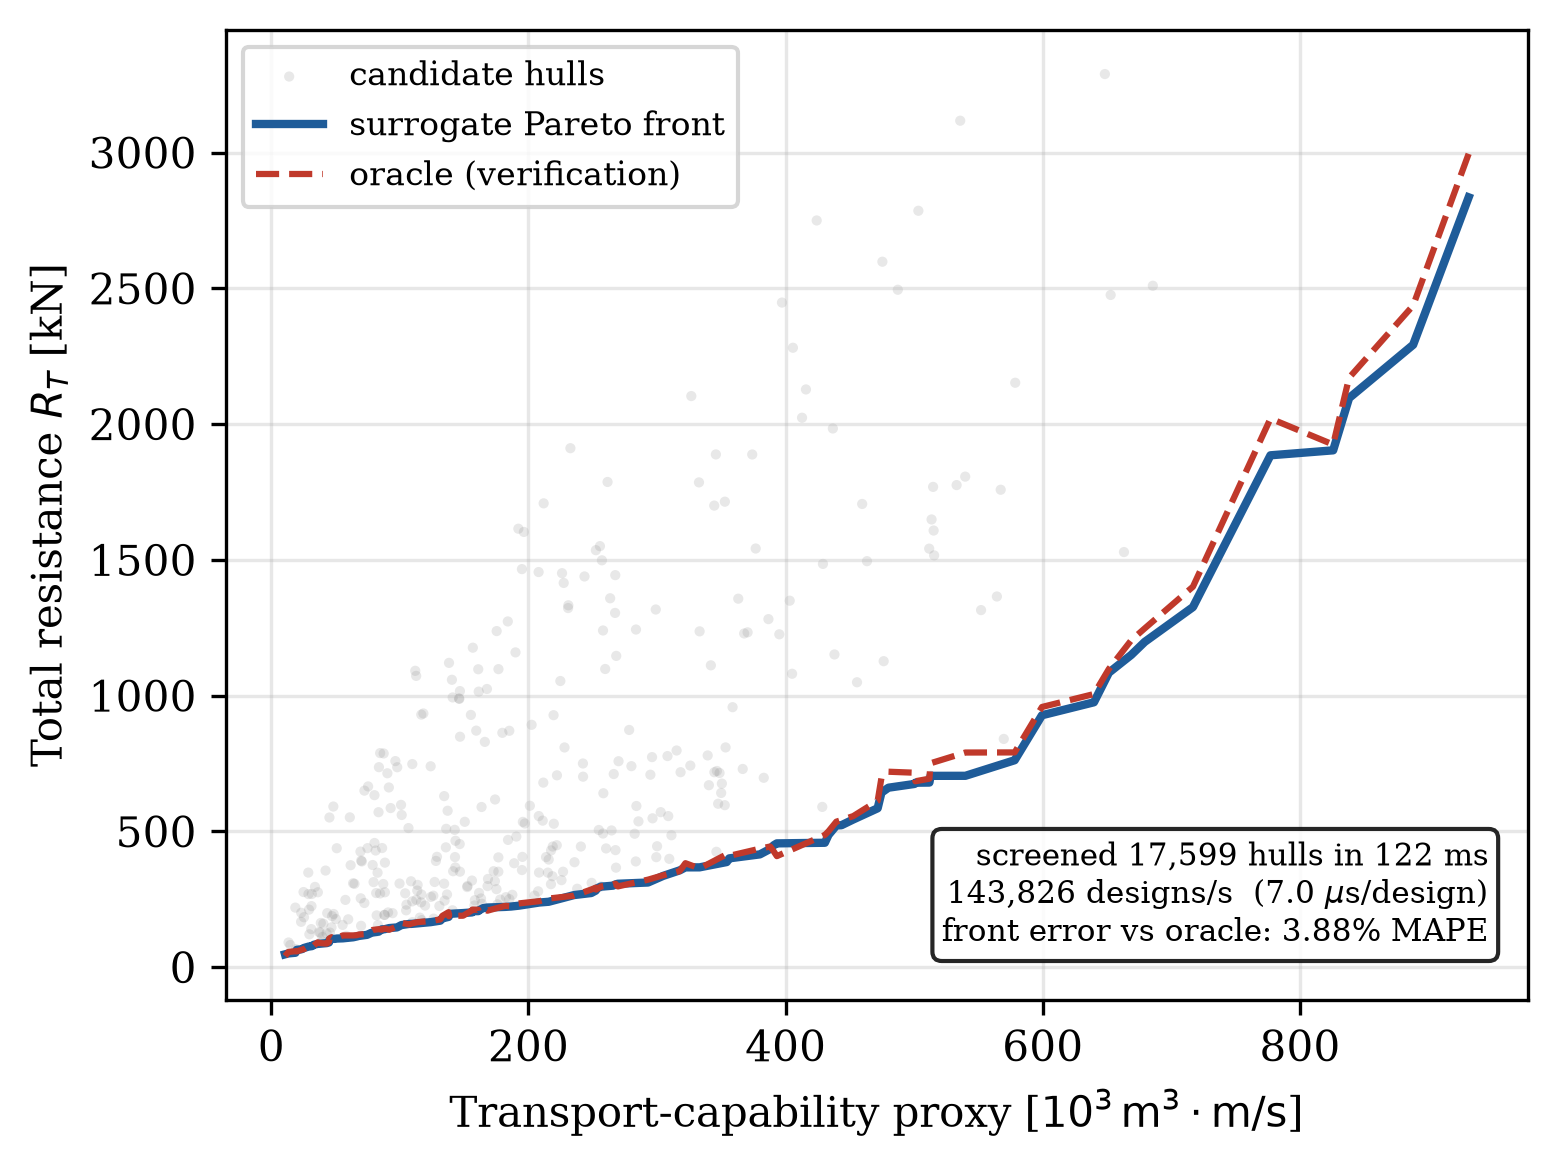
\includegraphics[width=0.68\textwidth]{figures/fig6_pareto.png}
\caption{Multi-objective design exploration. Grey: screened candidate hulls.
Blue: surrogate resistance--capability Pareto front. Dashed red: the same front
members re-evaluated with the ground-truth oracle. The surrogate screens about
144{,}000 designs per second and the front is faithful to within 3.9\%
MAPE.}\label{fig:pareto}
\end{figure}

The significance is in the throughput, not in beating the analytic oracle---
which, being a cheap correlation, is itself fast. The relevant baseline is
high-fidelity evaluation. A single steady RANS resistance computation is
conservatively of order a few CPU-hours; at 7 microseconds per design the
surrogate performs the equivalent screening $\mathcal{O}(10^{9})$ times faster
per query, turning a design sweep that would be wholly infeasible with direct
CFD (17{,}599 hulls $\times$ several CPU-hours $=$ years of compute) into a
sub-second interactive operation. This is the concrete mechanism by which ML
widens the early-stage design search---and, through it, the space of
resistance-optimal, lower-emission hulls a designer can consider under
EEDI/EEXI pressure.

\section{Broader roadmap: ML across naval architecture, ocean engineering and
shipbuilding}\label{sec:roadmap}

The resistance surrogate is one node in a larger, tractable programme.
Table~\ref{tab:roadmap} maps representative ML tasks across the three domains
onto their typical data modality and learning paradigm, and we highlight the
threads most tightly coupled to this work.

\begin{table}[h]
\caption{A map of machine-learning opportunities across the maritime design and
production lifecycle.}\label{tab:roadmap}
\centering
\begin{tabular}{@{}lll@{}}
\toprule
Domain & Task & Data / paradigm \\
\midrule
\multirow{3}{*}{Naval architecture}
 & Resistance \& power surrogacy (this work) & Principal particulars / regression \\
 & Hull-form shape optimisation              & Parametric geometry / Bayesian opt. \\
 & Seakeeping \& added resistance            & Wave spectra / sequence models \\
\midrule
\multirow{3}{*}{Ocean engineering}
 & Metocean \& wave forecasting              & Buoy, reanalysis / time-series \\
 & Trajectory \& motion prediction           & AIS, IMU / RNN, attention \\
 & Wave--structure interaction               & Field data / physics-informed NN \\
\midrule
\multirow{3}{*}{Shipbuilding}
 & Weld \& coating inspection                & Images, acoustic / CNN \\
 & Machinery predictive maintenance          & Sensor telemetry / anomaly det. \\
 & Assembly scheduling \& logistics          & Operations data / RL, opt. \\
\botrule
\end{tabular}
\end{table}

\paragraph{Uncertainty-aware active learning}
The learning curve of Fig.~\ref{fig:lc} and the GP's calibrated variance combine
naturally into an active-learning loop that minimises the number of costly
high-fidelity labels. Starting from a small design of experiments, the GP
proposes the next hull to evaluate where its predictive variance (or an
expected-improvement acquisition) is largest, the oracle/CFD labels it, and the
surrogate is updated. This is the standard route to CFD-call reductions of one
to two orders of magnitude in hull-form optimisation~\cite{serani2016,liu2022},
and our results---strong GP accuracy from 1200 points, steep early learning
curve---indicate the ingredients are in place.

\paragraph{Physics-informed and multi-fidelity surrogates}
Embedding known invariants (Reynolds and Froude scaling, monotonicity of
resistance in speed) as soft constraints, or fusing cheap empirical labels with
sparse RANS labels in a multi-fidelity GP, would improve data efficiency and
out-of-distribution behaviour beyond what a purely data-driven fit
achieves~\cite{raissi2019}.

\paragraph{From design to lifecycle}
A calibrated resistance-and-power surrogate is a reusable performance layer for a
vessel digital twin, queried downstream by voyage-optimisation, condition
monitoring and EEXI/CII compliance tools~\cite{major2021}. The same surrogate
methodology transfers to the shipbuilding tasks in Table~\ref{tab:roadmap},
where the expensive evaluator is a physical inspection or a production trial
rather than a CFD run.

\section{Limitations and threats to validity}\label{sec:limits}

Three limitations bound the claims above. First, the labels come from a
semi-empirical oracle rather than RANS CFD or tank tests; the reported
accuracies therefore measure the surrogate's ability to learn that oracle, not
absolute hydrodynamic fidelity. The methodology, protocol and throughput
conclusions transfer to high-fidelity labels, but the specific error numbers
would change with the label source, and validating on a genuine
CFD/experimental corpus is the essential next step. Second, the design space is
restricted to single-screw displacement hulls in calm water within
$F_n\le0.42$; planing craft, multihulls, appendage and propulsion effects, and
added resistance in a seaway are out of scope and would require additional
descriptors. Third, the transport-capability objective is a deliberately simple
proxy; a production study would substitute a proper deadweight/stability
estimate and add regulatory (EEDI) and cost objectives, turning the bi-objective
sweep into a constrained many-objective optimisation. None of these undermines
the paper's core finding---that modern regressors learn the resistance map to
below 2\% MAPE and enable design-space screening orders of magnitude faster than
high-fidelity evaluation---but each marks the boundary of what the present
experiments establish.

\section{Conclusion}\label{sec:conclusion}

We presented a reproducible machine-learning surrogate framework for
early-stage ship-hull resistance prediction and used it to drive large-scale
multi-objective design exploration. On a Latin-Hypercube-sampled dataset of 5232
feasible displacement hulls, non-linear regressors---gradient boosting, an MLP
and a Gaussian process---predict total resistance with $R^{2}$ up to 0.999 and
MAPE below 2\%, remaining stable under cross-validation, while a linear baseline
fails ($R^{2}=0.853$), confirming the strongly non-linear character of the map.
Analysing the accuracy--latency trade-off, we recommend gradient boosting or the
MLP for high-throughput screening and the Gaussian process where its calibrated
uncertainty is worth its cubic cost. Exercised as intended, the gradient-boosting
surrogate screens about 144{,}000 hulls per second and recovers a
resistance--capability Pareto front faithful to the oracle within 3.9\% MAPE---an
evaluation throughput orders of magnitude beyond direct CFD, and a concrete lever
for exploring lower-emission hulls under tightening efficiency regulation.
Future work follows directly from the roadmap of Section~\ref{sec:roadmap}:
retraining and validating the framework on a RANS/tank-test corpus; closing an
uncertainty-driven active-learning loop to minimise high-fidelity label cost;
incorporating physics-informed constraints and multi-fidelity fusion; and
extending the objective set to full EEDI-constrained, cost-aware many-objective
optimisation embedded in a vessel digital twin.

\backmatter

\bmhead{Supplementary information}
The semi-empirical oracle, the data-generation and experiment scripts, the
figure-generation code and the resulting dataset and metrics are provided in the
accompanying repository. All randomness is seeded, so every number, table and
figure in this paper is regenerable.

\section*{Declarations}

\begin{itemize}
\item \textbf{Funding.} Not applicable.
\item \textbf{Conflict of interest.} The authors declare that they have no
competing interests.
\item \textbf{Ethics approval and consent to participate.} Not applicable.
\item \textbf{Consent for publication.} Not applicable.
\item \textbf{Data availability.} The generated dataset is available in the
accompanying repository and can be regenerated from the provided seeded scripts.
\item \textbf{Materials availability.} Not applicable.
\item \textbf{Code availability.} All code (resistance oracle, data generation,
model training and figure generation) is provided in the accompanying repository.
\item \textbf{Author contribution.} All authors contributed to the study
conception, methodology, experiments and manuscript preparation.
\end{itemize}

\bibliography{references}

\end{document}
